%% Einleitung.tex
%% $Id: einleitung.tex 28 2007-01-18 16:31:32Z bless $
%%

\chapter{Einführung}
\label{ch:Introduction}
Bevor die für das Verständnis dieser Arbeit erforderlichen Details erklärt werden, wird auf das Problem der aktuellen Diagnose eines Atemaussetzers eingegangen. 
Anschließend wird die Idee beschrieben, wie dieses Problem in dieser Bachelorarbeit nun behandelt wird.
Zuletzt wird die Struktur der Vorangehensweise beschrieben, um einen Einblick zu geben, welchen Umfang die Bachelorarbeit hat.

\section{Problem}
Das in dieser Bachelorarbeit zu lösende Problem ist die Klassifizierung eines Atem"-aus"-set"-zers, welcher in verschiedenen Typen auftreten kann. 
In Abbildung \ref{introduction:problem_description} sind drei verschiedene Atmungsabläufe dargestellt. 
Darunter ist der jeweilige Atemfluss als Signal des zugehörigen Atemwegs abgebildet.
Bei verengten und geschlossenen Atemwegen ist eine deutliche Signaländerung vorhanden. 
Der Standard zur Diagnose eines solchen respiratorischen Ereignisses während des Schlafs ist eine Analyse in einem Schlaflabor mittels vieler angeschlossener Sensoren. 
Da man oft bis zu drei Monate auf einen Termin warten muss und die Untersuchung sehr kostspielig ist, hätte eine bequem von Zuhause aus durchführbare Alternative viele Vorteile.


\begin{figure}[h]
  \centering
  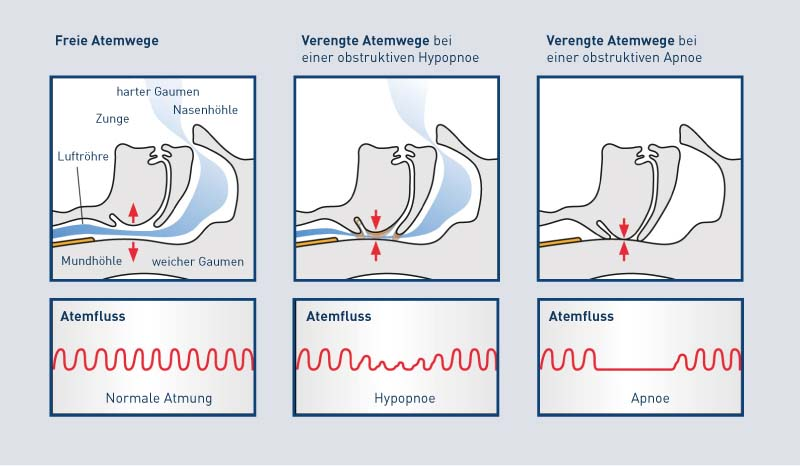
\includegraphics[width=0.55\textwidth]{introduction/was-passiert-bei-schlafapnoe}  
  \caption{Die Darstellung zeigt die Querschnittsansicht einer Person und derer Atemwege. Darunter ist der Atemfluss als Signal, welches Veränderungen während einer Atmungsstörung zeigt \cite{DeutscheFamilienversicherungSchlafapnoesyndrom}.}
  \label{introduction:problem_description}
\end{figure}

\newpage

\section{Idee}
Die Idee ist nun solche Signaleinbrüche mit maschinellem Lernen zu erkennen (siehe Abb. \ref{introduction:problem_description}). 
Das Signal wird durch eine IMU (\textit{inertial measurement unit}) der eSense-Earpods geliefert.
Dieses Signal besteht aus 6-Achsen, den \textit{x-}, \textit{y-} und \textit{z}-Achsen des Gyroskop- und Beschleunigungssensors.
Durch eine Klassifikation, also ob in einem Zeitintervall ein Apnoeereignis vorgekommen ist, oder nicht, kann eine erste Diagnose eines respiratorischen Ereignisses bereits bequem von Zuhause aus erfolgen.
Da der Proband eine Messung mit den eSense-Earpods über viele Nächte durchführen kann, sind die Signale über einen deutlich längeren Zeitabschnitt verfügbar, als sie in einem Schlaflabor aufgezeichnet werden.

\section{Struktur}
Zu Beginn wird eine App konstruiert, welche sich mit den eSense-Earpods über BLE (\textit{Bluetooth Low Energy}) verbindet (siehe Abb. \ref{introduction:ba_record}).
Anschließend wird eine Nutzerstudie mit 7 Personen durchgeführt, um einen Datensatz zu generieren.
Den Probanden wird über die Lautsprecher der eSense-Earpods mitgeteilt, wenn sie die Luft anhalten sollen, um eine zentrale Apnoe zu simulieren.
Anhand dieses Datensatzes kann schlussendlich ein Klassifikator trainiert werden, womit eine zukünftige Voraussage einer Messung getroffen werden kann.
Im dritten Bild der Abbildung \ref{introduction:ba_record} sind das Signal des PSG-Geräts und die Rohdaten der eSense-Earpods dargestellt. 
Zusammen bilden diese Signale neben den Kameraaufnahmen, dem Mikrofonsignal und den Nutzerinformationen einen Datensatz.
Das vierte Bild zeigt, dass nach der Klassifikation der Rohdaten, also der Gyroskop- und Beschleunigungsdaten der eSense-Earpods, eine Entscheidung darüber getroffen wird, ob in der Messung ein Apnoeereignis stattfand, oder nicht.
Die Messung wurde hierbei in viele Intervalle aufgeteilt, worauf jeweils eine individuelle Entscheidung getroffen wurde.

\begin{figure}[h]
  \centering
  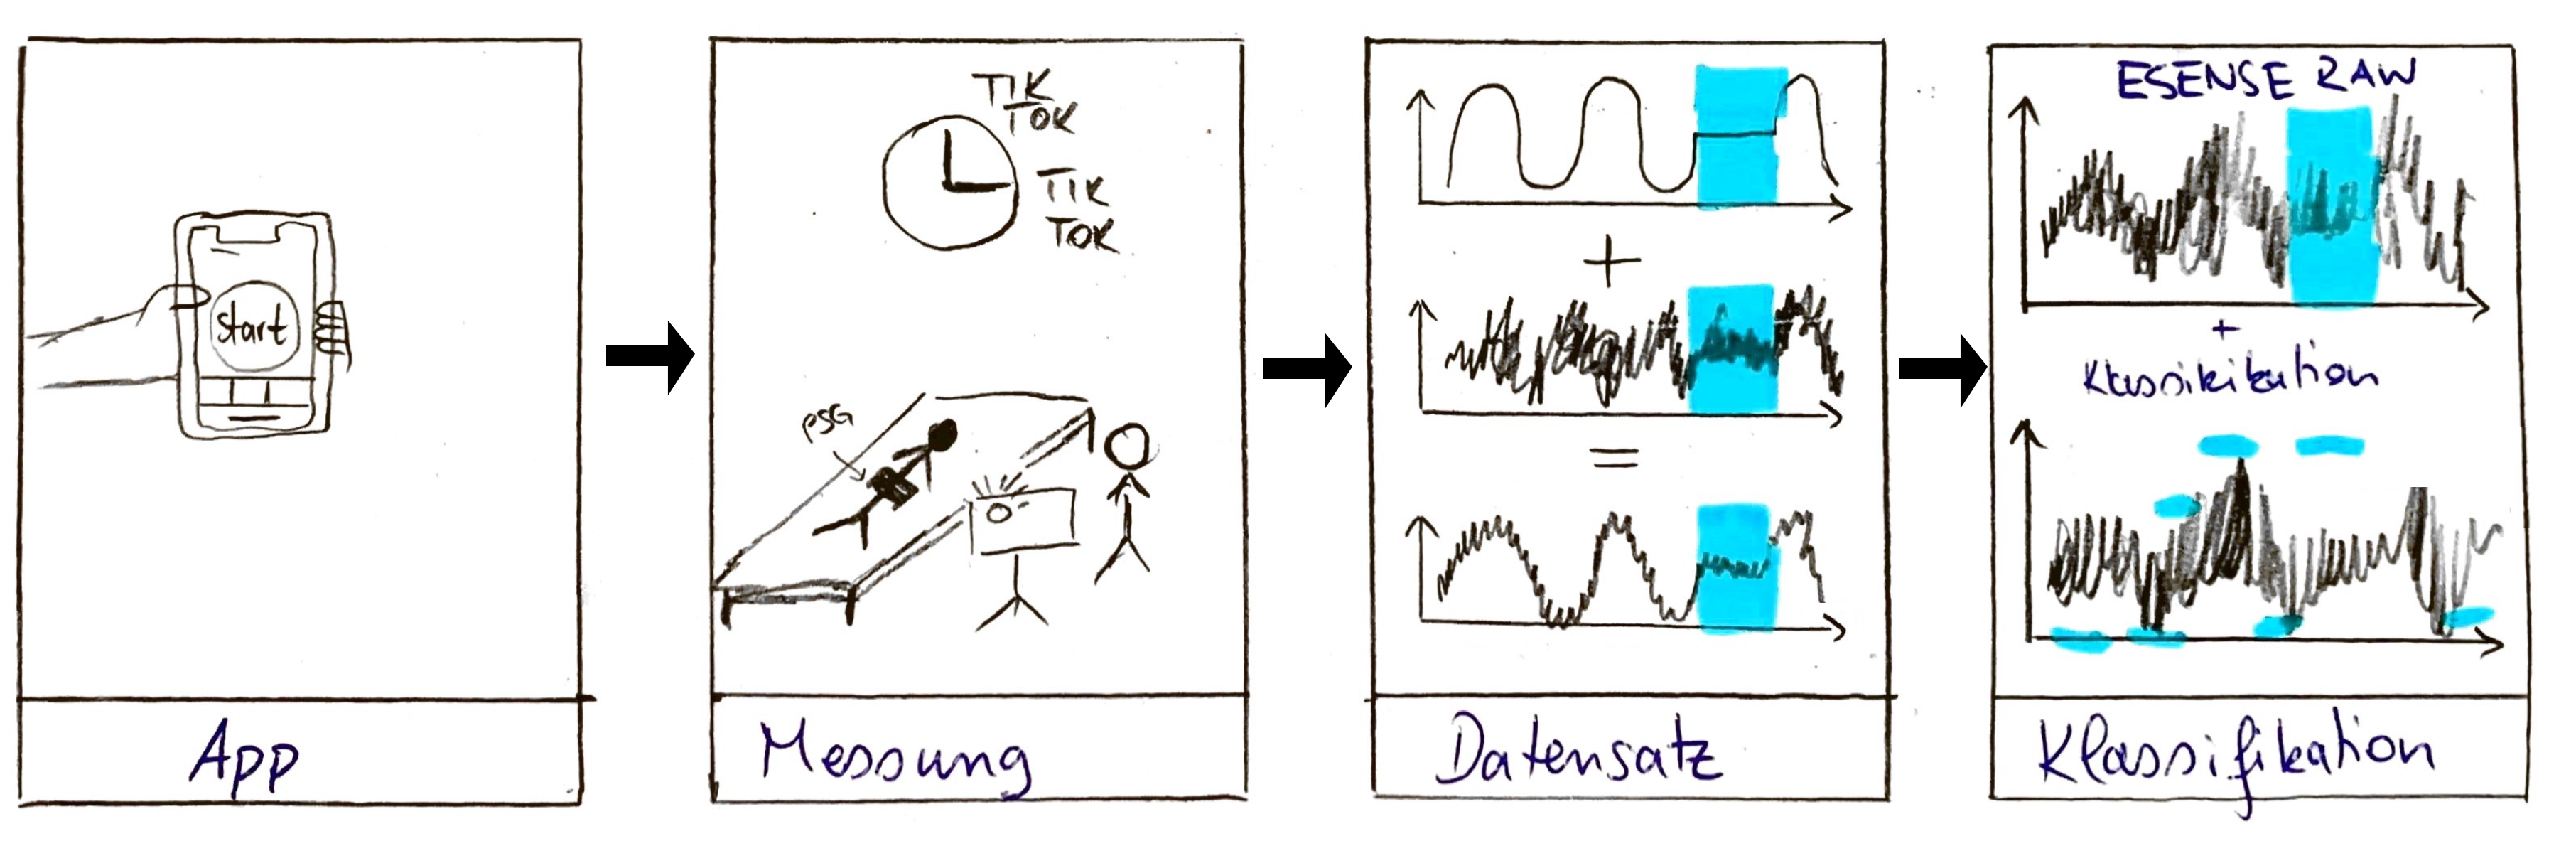
\includegraphics[width=1\textwidth]{ba_record_2}
  \caption{Darstellung des Ablaufs der Bachelorarbeit: Zu Beginn soll eine App erstellt werden, welche anschließend zur Datensammlung einer Nutzerstudie dient. Daraufhin wird ein Datensatz erstellt, welcher neben den Daten der eSense-Earpods auch den Ground-Truth beinhaltet. Anschließend wird eine Klassifikation anhand der Rohdaten der eSense-Earpods getroffen, ob ein Apnoeereignis in einem Intervall vorkommt, oder nicht.}
  \label{introduction:ba_record}
\end{figure}